\documentclass[12pt]{article}
\usepackage[utf8]{inputenc}
\usepackage{amsmath,amsthm,amsfonts,amssymb}
\usepackage{tikz}
\usepackage{subfig}
\usepackage[english]{babel}
\usepackage{capt-of}
\newtheorem{theorem}{Theorem}
\usetikzlibrary{calc}
\usetikzlibrary{shapes}
\usepackage{hyperref}
%might be unnecessary
\usepackage{doi}

%bibliography CMDS

%\usepackage{cite}
%\usepackage[style=alphabetic]{biblatex}
%\bibliographystyle{plain}

%\usepackage[style=alphabetic]{biblatex}

\usepackage[backend=biber,style=alphabetic]{biblatex}
%\usepackage[backend=bibtex,style=alphabetic]{biblatex}
\addbibresource{bibb.bib}

%%% With amsthm package, creates environments for nicely formatted,
%%% labeled, and numbered propositions, etc.
\theoremstyle{plain}
\newtheorem{thm}{Theorem}
\newtheorem{lemma}[thm]{Lemma}
\newtheorem{prop}[thm]{Proposition}
\newtheorem{conj}[thm]{Conjecture}
\newtheorem{cor}[thm]{Corollary}
\newtheorem{claim}[thm]{Claim}
\newtheorem{fact}[thm]{Fact}
\newtheorem{constraint}[thm]{Constraint}

\theoremstyle{definition}
\newtheorem{eg}[thm]{Example}
\newtheorem{defn}[thm]{Definition}
\newtheorem{rem}[thm]{Remark}
\newtheorem{observ}[thm]{Observation}
\newtheorem{open}[thm]{Open Problem}
\newtheorem{prob.}[thm]{Problem}
\newtheorem{quest}[thm]{Question}

% I used these for making definitions and theorems, not what is above
\theoremstyle{remark}
\newtheorem{remark}[thm]{Remark}
\newtheorem{note}[thm]{Note}
\theoremstyle{definition}
\newtheorem{definition}{Definition}[section]
\newtheorem{exmp}{Example}[section]

%custom commands

% blank cell
\newcommand{\cell}[4]{ \draw[thick] ( #1 , #2 ) rectangle ( #3 , #4 );}

% open cell 
\newcommand{\cellopen}[4]{ \draw[thick] ( #1 , #2 ) rectangle ( #3 , #4 ); \node[shape=circle,draw=red,fill=red, inner sep=0pt,minimum size=3pt] (A) at ( #1 * 0.5 + #3 * 0.5 , #2 * 0.5 + #4 * 0.5 ){};}

% /
\newcommand{\cellA}[4]{ \draw[thick] ( #1 , #2 ) rectangle ( #3 , #4 ); \draw[red, thick] (#3 * 0.5 + #1 * 0.5 , #2) -- (#3, #4 * 0.5 + #2 * 0.5);}

% \
\newcommand{\cellB}[4]{ \draw[thick] ( #1 , #2 ) rectangle ( #3 , #4 ); \draw[red, thick] (#3 * 0.5 + #1 * 0.5 , #2) -- (#1, #4 * 0.5 + #2 * 0.5);}

% /
\newcommand{\cellC}[4]{ \draw[thick] ( #1 , #2 ) rectangle ( #3 , #4 ); \draw[red, thick] (#3 * 0.5 + #1 * 0.5 , #4) -- (#1, #4 * 0.5 + #2 * 0.5);}

% L
\newcommand{\cellD}[4]{ \draw[thick] ( #1 , #2 ) rectangle ( #3 , #4 ); \draw[red, thick] (#3 * 0.5 + #1 * 0.5 , #4) -- (#3, #4 * 0.5 + #2 * 0.5);}

% |
\newcommand{\cellE}[4]{ \draw[thick] ( #1 , #2 ) rectangle ( #3 , #4 ); \draw[red, thick] (#3 * 0.5 + #1 * 0.5 , #2) -- (#3 * 0.5 + #1 * 0.5 , #4);}

% -
\newcommand{\cellF}[4]{ \draw[thick] ( #1 , #2 ) rectangle ( #3 , #4 ); \draw[red, thick] (#3, #4 * 0.5 + #2 * 0.5) -- (#1, #4 * 0.5 + #2 * 0.5);}

\newcommand{\cellAf}[4]{\filldraw[gray!40] ( #1 , #2 ) rectangle ( #3 , #4 ); \draw[thick] ( #1 , #2 ) rectangle ( #3 , #4 ); \draw[red, thick] (#3 * 0.5 + #1 * 0.5 , #2) -- (#3, #4 * 0.5 + #2 * 0.5);}

% \
\newcommand{\cellBf}[4]{\filldraw[gray!40] ( #1 , #2 ) rectangle ( #3 , #4 ); \draw[thick] ( #1 , #2 ) rectangle ( #3 , #4 ); \draw[red, thick] (#3 * 0.5 + #1 * 0.5 , #2) -- (#1, #4 * 0.5 + #2 * 0.5);}

% /
\newcommand{\cellCf}[4]{\filldraw[gray!40] ( #1 , #2 ) rectangle ( #3 , #4 ); \draw[thick] ( #1 , #2 ) rectangle ( #3 , #4 ); \draw[red, thick] (#3 * 0.5 + #1 * 0.5 , #4) -- (#1, #4 * 0.5 + #2 * 0.5);}

% L
\newcommand{\cellDf}[4]{\filldraw[gray!40] ( #1 , #2 ) rectangle ( #3 , #4 ); \draw[thick] ( #1 , #2 ) rectangle ( #3 , #4 ); \draw[red, thick] (#3 * 0.5 + #1 * 0.5 , #4) -- (#3, #4 * 0.5 + #2 * 0.5);}

% |
\newcommand{\cellEf}[4]{\filldraw[gray!40] ( #1 , #2 ) rectangle ( #3 , #4 ); \draw[thick] ( #1 , #2 ) rectangle ( #3 , #4 ); \draw[red, thick] (#3 * 0.5 + #1 * 0.5 , #2) -- (#3 * 0.5 + #1 * 0.5 , #4);}

% -
\newcommand{\cellFf}[4]{\filldraw[gray!40] ( #1 , #2 ) rectangle ( #3 , #4 ); \draw[thick] ( #1 , #2 ) rectangle ( #3 , #4 ); \draw[red, thick] (#3, #4 * 0.5 + #2 * 0.5) -- (#1, #4 * 0.5 + #2 * 0.5);}


\newcommand{\lablnode}[3]{\node[shape=circle,draw=none,fill=none, inner sep=0pt,minimum size=0pt] (A) at ( #1 , #2 ) {#3};}

\usepackage[margin=1in]{geometry}

%doc info
\title{The Mosaic Problem}
\author{Richard Shank, Jack Hanke}
\date{\today}

\begin{document}

\begin{center}
    \Large
    \textbf{The Mosaic Problem}
    
    \vspace{0.4cm}
    \large
    
    Richard Shank, Jack Hanke   
    \vspace{0.4cm}
    
    \today
    \vspace{0.4cm}    
\end{center}

\section{Introduction}

Consider the following $6$ unit squares with markings on them.

%figure of tiles (colored marknigs!)
\begin{center}
    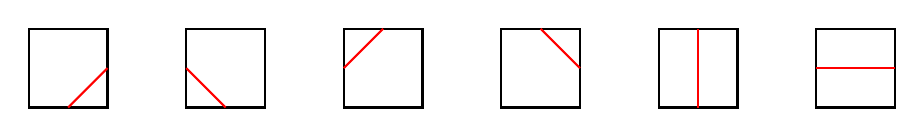
\begin{tikzpicture}
    \cellA{0}{0}{1}{1}
    \cellB{2}{0}{3}{1}
    \cellC{4}{0}{5}{1}
    \cellD{6}{0}{7}{1}
    \cellE{8}{0}{9}{1}
    \cellF{10}{0}{11}{1}    
    \end{tikzpicture}
\end{center}

Call these squares \textit{tiles}. 

\begin{definition}
An $(n,m)$-\textit{mosaic} is an $(n,m)$ rectangular lattice made up of tiles.
\end{definition}

\begin{exmp}
An example of a $(7,5)$-mosaic:
\begin{center}
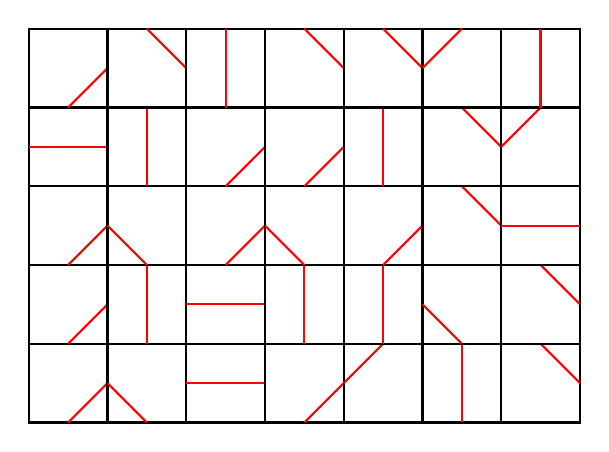
\begin{tikzpicture}
    % row1
    \cellA{0}{0}{1}{1}
    \cellB{1}{0}{2}{1}
    \cellF{2}{0}{3}{1}
    \cellA{3}{0}{4}{1}
    \cellC{4}{0}{5}{1}
    \cellE{5}{0}{6}{1}
    \cellD{6}{0}{7}{1}
    % row2
    \cellA{0}{1}{1}{2}
    \cellE{1}{1}{2}{2}
    \cellF{2}{1}{3}{2}
    \cellE{3}{1}{4}{2}
    \cellE{4}{1}{5}{2}
    \cellB{5}{1}{6}{2}
    \cellD{6}{1}{7}{2}
    % row3
    \cellA{0}{2}{1}{3}
    \cellB{1}{2}{2}{3}
    \cellA{2}{2}{3}{3}
    \cellB{3}{2}{4}{3}
    \cellA{4}{2}{5}{3}
    \cellD{5}{2}{6}{3}
    \cellF{6}{2}{7}{3}
    % row4
    \cellF{0}{3}{1}{4}
    \cellE{1}{3}{2}{4}
    \cellA{2}{3}{3}{4}
    \cellA{3}{3}{4}{4}
    \cellE{4}{3}{5}{4}
    \cellD{5}{3}{6}{4}
    \cellC{6}{3}{7}{4}
    % row5
    \cellA{0}{4}{1}{5}
    \cellD{1}{4}{2}{5}
    \cellE{2}{4}{3}{5}
    \cellD{3}{4}{4}{5}
    \cellD{4}{4}{5}{5}
    \cellC{5}{4}{6}{5}
    \cellE{6}{4}{7}{5}
\end{tikzpicture}
\end{center}
\end{exmp}

Clearly there are $6^{nm}$ possible mosaics. Which of these mosaics contain self-avoiding polygons?

%example of a mosaic with an enclosed region
\begin{exmp}
\label{exp:sap}
An example of a $(7,5)$-mosaic with a self-avoiding polygon, hilighted in gray:
\begin{center}
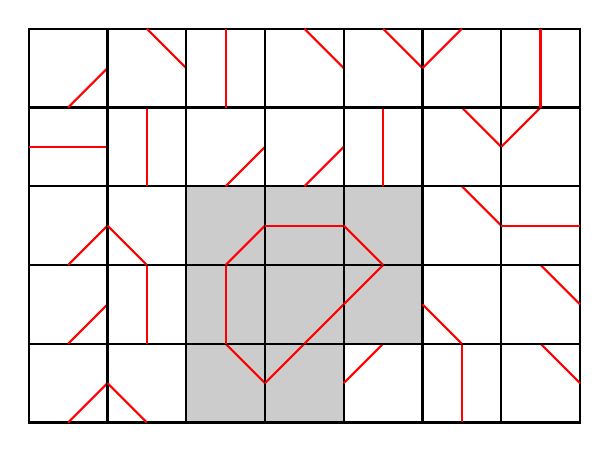
\begin{tikzpicture}
    % row1
    \cellA{0}{0}{1}{1}
    \cellB{1}{0}{2}{1}
    \cellDf{2}{0}{3}{1}
    \cellCf{3}{0}{4}{1}
    \cellC{4}{0}{5}{1}
    \cellE{5}{0}{6}{1}
    \cellD{6}{0}{7}{1}
    % row2
    \cellA{0}{1}{1}{2}
    \cellE{1}{1}{2}{2}
    \cellEf{2}{1}{3}{2}
    \cellAf{3}{1}{4}{2}
    \cellCf{4}{1}{5}{2}
    \cellB{5}{1}{6}{2}
    \cellD{6}{1}{7}{2}
    % row3
    \cellA{0}{2}{1}{3}
    \cellB{1}{2}{2}{3}
    \cellAf{2}{2}{3}{3}
    \cellFf{3}{2}{4}{3}
    \cellBf{4}{2}{5}{3}
    \cellD{5}{2}{6}{3}
    \cellF{6}{2}{7}{3}
    % row4
    \cellF{0}{3}{1}{4}
    \cellE{1}{3}{2}{4}
    \cellA{2}{3}{3}{4}
    \cellA{3}{3}{4}{4}
    \cellE{4}{3}{5}{4}
    \cellD{5}{3}{6}{4}
    \cellC{6}{3}{7}{4}
    % row5
    \cellA{0}{4}{1}{5}
    \cellD{1}{4}{2}{5}
    \cellE{2}{4}{3}{5}
    \cellD{3}{4}{4}{5}
    \cellD{4}{4}{5}{5}
    \cellC{5}{4}{6}{5}
    \cellE{6}{4}{7}{5}
\end{tikzpicture}
\end{center}
\end{exmp}

Let $t_{n,m}$ be the number of mosaics that have at least one self avoiding polygon (SAP). Clearly $t_{n,m}=t_{m,n}.$ Also from the fact that the smallest SAP is

\begin{center}
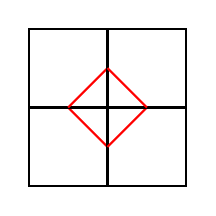
\begin{tikzpicture}
% row1
\cellD{0}{0}{1}{1}
\cellC{1}{0}{2}{1}
% row2
\cellA{0}{1}{1}{2}
\cellB{1}{1}{2}{2}
\end{tikzpicture}
\end{center}

we have that $t_{n,1}=t_{1,m}=0$, and $t_{2,2} = 1$. What else can be said?

\begin{thm}

Assume $n \geq m $

$$
M(m) = \begin{bmatrix}
36 & 1 \\
-1 & 1
\end{bmatrix}
$$

For $h \geq 2$, then if
$$
M(m) = \begin{bmatrix}
M_1 & M_2 \\
M_3 & M_4
\end{bmatrix}
$$

then
$$
M(m+1) = \begin{bmatrix}
6M_1 & 6M_2 & \frac{1}{6}M_1 & 1M_2 \\
6M_3 & 6M_4 & 0M_3 & 1M_4 \\
-\frac{1}{6}M_1 & 0M_2 & \frac{1}{6}M_1 & 1M_2 \\
1M_3 & 1M_4 & -1M_3 & 6M_4 \\
\end{bmatrix}
$$

where $M_i$ is a sub-matrix of the block matrix $M$.

Then for the given $m$, define the rows and columns of $M(m)$ as

$$
M(m) = 
\begin{bmatrix}
    c_1 & c_2 & ... & c_{2^{m-1}}
\end{bmatrix} = 
\begin{bmatrix}
    r_1 \\
    r_2 \\
    ... \\
    r_{2^{m-1}} \\
\end{bmatrix}
$$

Then let $v,L(n) \in \mathbb{R}^{2^{m-1} \times 1}$ so that

$$v_i = -1*r_i \cdot c_1$$
excluding the first term of the dot product,

and
$$L(n) = M(m) \cdot L(n-1)+v$$

Then $t_{n,m}=r_1 \cdot (M(m) \cdot L(n-1)+v).$

\end{thm}

\begin{proof}
Begin by labelling the vertices of the rectangular lattice as follows. If the vertex is surrounded by an even number of SAPs, color it black. If the vertex is surrounded by an odd number of SAPs, color it green. Using the mosaic from Example \ref{exp:sap}, we get the following labelling.

\begin{center}
    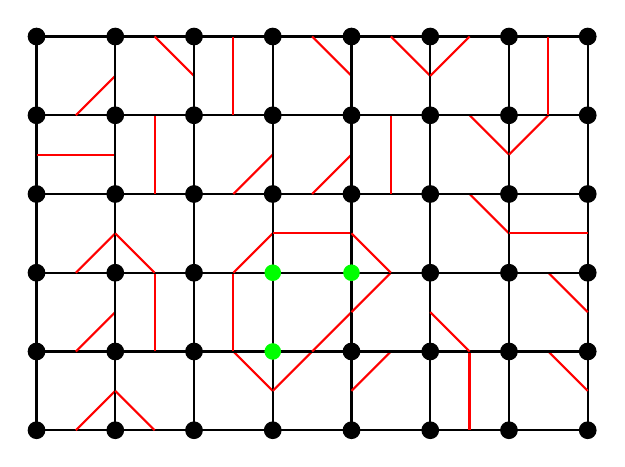
\begin{tikzpicture}
        % row1
        \cellA{0}{0}{1}{1}
        \cellB{1}{0}{2}{1}
        \cellD{2}{0}{3}{1}
        \cellC{3}{0}{4}{1}
        \cellC{4}{0}{5}{1}
        \cellE{5}{0}{6}{1}
        \cellD{6}{0}{7}{1}
        % row2
        \cellA{0}{1}{1}{2}
        \cellE{1}{1}{2}{2}
        \cellE{2}{1}{3}{2}
        \cellA{3}{1}{4}{2}
        \cellC{4}{1}{5}{2}
        \cellB{5}{1}{6}{2}
        \cellD{6}{1}{7}{2}
        % row3
        \cellA{0}{2}{1}{3}
        \cellB{1}{2}{2}{3}
        \cellA{2}{2}{3}{3}
        \cellF{3}{2}{4}{3}
        \cellB{4}{2}{5}{3}
        \cellD{5}{2}{6}{3}
        \cellF{6}{2}{7}{3}
        % row4
        \cellF{0}{3}{1}{4}
        \cellE{1}{3}{2}{4}
        \cellA{2}{3}{3}{4}
        \cellA{3}{3}{4}{4}
        \cellE{4}{3}{5}{4}
        \cellD{5}{3}{6}{4}
        \cellC{6}{3}{7}{4}
        % row5
        \cellA{0}{4}{1}{5}
        \cellD{1}{4}{2}{5}
        \cellE{2}{4}{3}{5}
        \cellD{3}{4}{4}{5}
        \cellD{4}{4}{5}{5}
        \cellC{5}{4}{6}{5}
        \cellE{6}{4}{7}{5}
        % label for row1
        \draw[fill=black] (0,0) circle (3pt);
        \draw[fill=black] (1,0) circle (3pt);
        \draw[fill=black] (2,0) circle (3pt);
        \draw[fill=black] (3,0) circle (3pt);
        \draw[fill=black] (4,0) circle (3pt);
        \draw[fill=black] (5,0) circle (3pt);
        \draw[fill=black] (6,0) circle (3pt);
        \draw[fill=black] (7,0) circle (3pt);
        % label for row1
        \draw[fill=black] (0,1) circle (3pt);
        \draw[fill=black] (1,1) circle (3pt);
        \draw[fill=black] (2,1) circle (3pt);
        \draw[fill=green, draw=none] (3,1) circle (3pt);
        \draw[fill=black] (4,1) circle (3pt);
        \draw[fill=black] (5,1) circle (3pt);
        \draw[fill=black] (6,1) circle (3pt);
        \draw[fill=black] (7,1) circle (3pt);
        % label for row1
        \draw[fill=black] (0,2) circle (3pt);
        \draw[fill=black] (1,2) circle (3pt);
        \draw[fill=black] (2,2) circle (3pt);
        \draw[fill=green, draw=none] (3,2) circle (3pt);
        \draw[fill=green, draw=none] (4,2) circle (3pt);
        \draw[fill=black] (5,2) circle (3pt);
        \draw[fill=black] (6,2) circle (3pt);
        \draw[fill=black] (7,2) circle (3pt);
        % label for row1
        \draw[fill=black] (0,3) circle (3pt);
        \draw[fill=black] (1,3) circle (3pt);
        \draw[fill=black] (2,3) circle (3pt);
        \draw[fill=black] (3,3) circle (3pt);
        \draw[fill=black] (4,3) circle (3pt);
        \draw[fill=black] (5,3) circle (3pt);
        \draw[fill=black] (6,3) circle (3pt);
        \draw[fill=black] (7,3) circle (3pt);
        % label for row1
        \draw[fill=black] (0,4) circle (3pt);
        \draw[fill=black] (1,4) circle (3pt);
        \draw[fill=black] (2,4) circle (3pt);
        \draw[fill=black] (3,4) circle (3pt);
        \draw[fill=black] (4,4) circle (3pt);
        \draw[fill=black] (5,4) circle (3pt);
        \draw[fill=black] (6,4) circle (3pt);
        \draw[fill=black] (7,4) circle (3pt);
        % label for row1
        \draw[fill=black] (0,5) circle (3pt);
        \draw[fill=black] (1,5) circle (3pt);
        \draw[fill=black] (2,5) circle (3pt);
        \draw[fill=black] (3,5) circle (3pt);
        \draw[fill=black] (4,5) circle (3pt);
        \draw[fill=black] (5,5) circle (3pt);
        \draw[fill=black] (6,5) circle (3pt);
        \draw[fill=black] (7,5) circle (3pt);
    \end{tikzpicture}
\end{center}

Notice that vertices on the boundary of the lattice will always be black. The associated \textit{parity configuration} for the above mosaic is below.

\begin{center}
    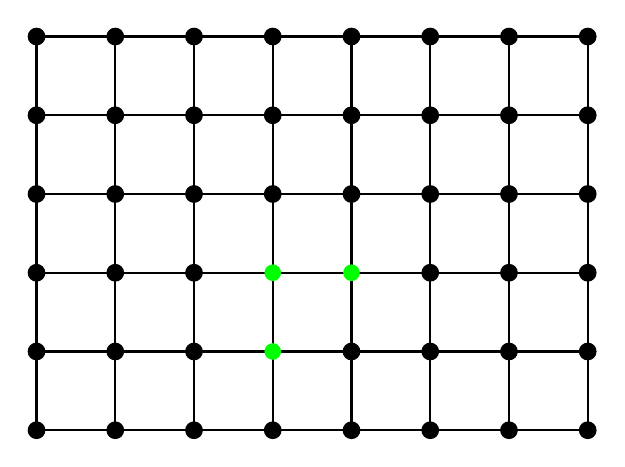
\begin{tikzpicture}
        % row1
        \cell{0}{0}{1}{1}
        \cell{1}{0}{2}{1}
        \cell{2}{0}{3}{1}
        \cell{3}{0}{4}{1}
        \cell{4}{0}{5}{1}
        \cell{5}{0}{6}{1}
        \cell{6}{0}{7}{1}
        % row2
        \cell{0}{1}{1}{2}
        \cell{1}{1}{2}{2}
        \cell{2}{1}{3}{2}
        \cell{3}{1}{4}{2}
        \cell{4}{1}{5}{2}
        \cell{5}{1}{6}{2}
        \cell{6}{1}{7}{2}
        % row3
        \cell{0}{2}{1}{3}
        \cell{1}{2}{2}{3}
        \cell{2}{2}{3}{3}
        \cell{3}{2}{4}{3}
        \cell{4}{2}{5}{3}
        \cell{5}{2}{6}{3}
        \cell{6}{2}{7}{3}
        % row4
        \cell{0}{3}{1}{4}
        \cell{1}{3}{2}{4}
        \cell{2}{3}{3}{4}
        \cell{3}{3}{4}{4}
        \cell{4}{3}{5}{4}
        \cell{5}{3}{6}{4}
        \cell{6}{3}{7}{4}
        % row5
        \cell{0}{4}{1}{5}
        \cell{1}{4}{2}{5}
        \cell{2}{4}{3}{5}
        \cell{3}{4}{4}{5}
        \cell{4}{4}{5}{5}
        \cell{5}{4}{6}{5}
        \cell{6}{4}{7}{5}
        % label for row1
        \draw[fill=black] (0,0) circle (3pt);
        \draw[fill=black] (1,0) circle (3pt);
        \draw[fill=black] (2,0) circle (3pt);
        \draw[fill=black] (3,0) circle (3pt);
        \draw[fill=black] (4,0) circle (3pt);
        \draw[fill=black] (5,0) circle (3pt);
        \draw[fill=black] (6,0) circle (3pt);
        \draw[fill=black] (7,0) circle (3pt);
        % label for row1
        \draw[fill=black] (0,1) circle (3pt);
        \draw[fill=black] (1,1) circle (3pt);
        \draw[fill=black] (2,1) circle (3pt);
        \draw[fill=green, draw=none] (3,1) circle (3pt);
        \draw[fill=black] (4,1) circle (3pt);
        \draw[fill=black] (5,1) circle (3pt);
        \draw[fill=black] (6,1) circle (3pt);
        \draw[fill=black] (7,1) circle (3pt);
        % label for row1
        \draw[fill=black] (0,2) circle (3pt);
        \draw[fill=black] (1,2) circle (3pt);
        \draw[fill=black] (2,2) circle (3pt);
        \draw[fill=green, draw=none] (3,2) circle (3pt);
        \draw[fill=green, draw=none] (4,2) circle (3pt);
        \draw[fill=black] (5,2) circle (3pt);
        \draw[fill=black] (6,2) circle (3pt);
        \draw[fill=black] (7,2) circle (3pt);
        % label for row1
        \draw[fill=black] (0,3) circle (3pt);
        \draw[fill=black] (1,3) circle (3pt);
        \draw[fill=black] (2,3) circle (3pt);
        \draw[fill=black] (3,3) circle (3pt);
        \draw[fill=black] (4,3) circle (3pt);
        \draw[fill=black] (5,3) circle (3pt);
        \draw[fill=black] (6,3) circle (3pt);
        \draw[fill=black] (7,3) circle (3pt);
        % label for row1
        \draw[fill=black] (0,4) circle (3pt);
        \draw[fill=black] (1,4) circle (3pt);
        \draw[fill=black] (2,4) circle (3pt);
        \draw[fill=black] (3,4) circle (3pt);
        \draw[fill=black] (4,4) circle (3pt);
        \draw[fill=black] (5,4) circle (3pt);
        \draw[fill=black] (6,4) circle (3pt);
        \draw[fill=black] (7,4) circle (3pt);
        % label for row1
        \draw[fill=black] (0,5) circle (3pt);
        \draw[fill=black] (1,5) circle (3pt);
        \draw[fill=black] (2,5) circle (3pt);
        \draw[fill=black] (3,5) circle (3pt);
        \draw[fill=black] (4,5) circle (3pt);
        \draw[fill=black] (5,5) circle (3pt);
        \draw[fill=black] (6,5) circle (3pt);
        \draw[fill=black] (7,5) circle (3pt);
    \end{tikzpicture}
\end{center}

Let $\mathcal{P} (n,m)$ denote all possible parity configurations for an $(n,m)$ rectangular lattice. Clearly $|\mathcal{P} (n,m)| = 2^{(n-1)(m-1)}$. Then let $f(p)$ be a function of a specific parity configuration that retuns the number of possible mosaics that map to $p$, multiplied by $-1$ to the number of SAPs specified by $p$. For example, the above parity configuration specifies only $1$ SAP, so $f(p) = -1 * 6^{28}$. 

Then one can write

$$t_{n,m} = -\sum_{p \in \mathcal{P}(n,m)}f(p).$$

Amazingly, $f(p)$ can be written as a product of some choice of weights $w_{1} , \dots, w_{16}$ associated with the following individual \textit{cell-parity configurations}.

\begin{center}
    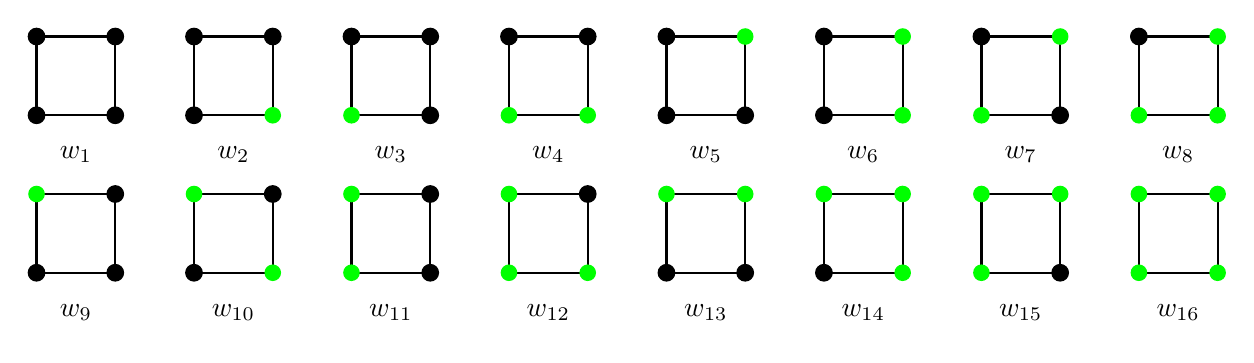
\begin{tikzpicture}
        % row1
        \cell{0}{0}{1}{1}
        \cell{2}{0}{3}{1}
        \cell{4}{0}{5}{1}
        \cell{6}{0}{7}{1}
        \cell{8}{0}{9}{1}
        \cell{10}{0}{11}{1}
        \cell{12}{0}{13}{1}
        \cell{14}{0}{15}{1}
        % row2
        \cell{0}{2}{1}{3}
        \cell{2}{2}{3}{3}
        \cell{4}{2}{5}{3}
        \cell{6}{2}{7}{3}
        \cell{8}{2}{9}{3}
        \cell{10}{2}{11}{3}
        \cell{12}{2}{13}{3}
        \cell{14}{2}{15}{3}
        % label for row1
        \draw[fill=black] (0,0) circle (3pt);
        \draw[fill=black] (1,0) circle (3pt);
        \draw[fill=black] (2,0) circle (3pt);
        \draw[fill=green, draw=none] (3,0) circle (3pt);
        \draw[fill=green, draw=none] (4,0) circle (3pt);
        \draw[fill=black] (5,0) circle (3pt);
        \draw[fill=green, draw=none] (6,0) circle (3pt);
        \draw[fill=green, draw=none] (7,0) circle (3pt);
        \draw[fill=black] (8,0) circle (3pt);
        \draw[fill=black] (9,0) circle (3pt);
        \draw[fill=black] (10,0) circle (3pt);
        \draw[fill=green, draw=none] (11,0) circle (3pt);
        \draw[fill=green, draw=none] (12,0) circle (3pt);
        \draw[fill=black] (13,0) circle (3pt);
        \draw[fill=green, draw=none] (14,0) circle (3pt);
        \draw[fill=green, draw=none] (15,0) circle (3pt);
        % label for row1
        \draw[fill=green, draw=none] (0,1) circle (3pt);
        \draw[fill=black] (1,1) circle (3pt);
        \draw[fill=green, draw=none] (2,1) circle (3pt);
        \draw[fill=black] (3,1) circle (3pt);
        \draw[fill=green, draw=none] (4,1) circle (3pt);
        \draw[fill=black] (5,1) circle (3pt);
        \draw[fill=green, draw=none] (6,1) circle (3pt);
        \draw[fill=black] (7,1) circle (3pt);
        \draw[fill=green, draw=none] (8,1) circle (3pt);
        \draw[fill=green, draw=none] (9,1) circle (3pt);
        \draw[fill=green, draw=none] (10,1) circle (3pt);
        \draw[fill=green, draw=none] (11,1) circle (3pt);
        \draw[fill=green, draw=none] (12,1) circle (3pt);
        \draw[fill=green, draw=none] (13,1) circle (3pt);
        \draw[fill=green, draw=none] (14,1) circle (3pt);
        \draw[fill=green, draw=none] (15,1) circle (3pt);
        % label for row1
        \draw[fill=black] (0,2) circle (3pt);
        \draw[fill=black] (1,2) circle (3pt);
        \draw[fill=black] (2,2) circle (3pt);
        \draw[fill=green, draw=none] (3,2) circle (3pt);
        \draw[fill=green, draw=none] (4,2) circle (3pt);
        \draw[fill=black] (5,2) circle (3pt);
        \draw[fill=green, draw=none] (6,2) circle (3pt);
        \draw[fill=green, draw=none] (7,2) circle (3pt);
        \draw[fill=black] (8,2) circle (3pt);
        \draw[fill=black] (9,2) circle (3pt);
        \draw[fill=black] (10,2) circle (3pt);
        \draw[fill=green, draw=none] (11,2) circle (3pt);
        \draw[fill=green, draw=none] (12,2) circle (3pt);
        \draw[fill=black] (13,2) circle (3pt);
        \draw[fill=green, draw=none] (14,2) circle (3pt);
        \draw[fill=green, draw=none] (15,2) circle (3pt);
        % label for row1
        \draw[fill=black] (0,3) circle (3pt);
        \draw[fill=black] (1,3) circle (3pt);
        \draw[fill=black] (2,3) circle (3pt);
        \draw[fill=black] (3,3) circle (3pt);
        \draw[fill=black] (4,3) circle (3pt);
        \draw[fill=black] (5,3) circle (3pt);
        \draw[fill=black] (6,3) circle (3pt);
        \draw[fill=black] (7,3) circle (3pt);
        \draw[fill=black] (8,3) circle (3pt);
        \draw[fill=green, draw=none] (9,3) circle (3pt);
        \draw[fill=black] (10,3) circle (3pt);
        \draw[fill=green, draw=none] (11,3) circle (3pt);
        \draw[fill=black] (12,3) circle (3pt);
        \draw[fill=green, draw=none] (13,3) circle (3pt);
        \draw[fill=black] (14,3) circle (3pt);
        \draw[fill=green, draw=none] (15,3) circle (3pt);
        % numbers row 1
        \( \lablnode{0.5}{-0.5}{$w_{9}$} \)
        \( \lablnode{2.5}{-0.5}{$w_{10}$} \)
        \( \lablnode{4.5}{-0.5}{$w_{11}$} \)
        \( \lablnode{6.5}{-0.5}{$w_{12}$} \)
        \( \lablnode{8.5}{-0.5}{$w_{13}$} \)
        \( \lablnode{10.5}{-0.5}{$w_{14}$} \)
        \( \lablnode{12.5}{-0.5}{$w_{15}$} \)
        \( \lablnode{14.5}{-0.5}{$w_{16}$} \)
        % numbers row 2
        \( \lablnode{0.5}{1.5}{$w_{1}$} \)
        \( \lablnode{2.5}{1.5}{$w_{2}$} \)
        \( \lablnode{4.5}{1.5}{$w_{3}$} \)
        \( \lablnode{6.5}{1.5}{$w_{4}$} \)
        \( \lablnode{8.5}{1.5}{$w_{5}$} \)
        \( \lablnode{10.5}{1.5}{$w_{6}$} \)
        \( \lablnode{12.5}{1.5}{$w_{7}$} \)
        \( \lablnode{14.5}{1.5}{$w_{8}$} \)
    \end{tikzpicture}
\end{center}

One can assign values to $w_{1},\dots,w_{16}$ so that the product for all parity configurations $p$ equals $f(p)$. To find these assignments, first notice that $w_{1} = w_{16} = 6$, as these cells do not indicate a specific tile. Similarly, $w_{7}=w_{10}=0$, as these are impossible parity configurations for our tile set. The remaining weights uniquely specify a tile, and so are equal to $1$ or $-1$. But how do we find these assignments?

First notice that we want a weight assignment so that the parity configurations for a given SAP multiply to $-1$. This means that if there are multiple SAPs in a mosaic, then the product will be positive if there is an even number of SAPs specified, and negative if there is an odd number specified.

Next note the following lemma.
\begin{lemma}
    \label{lemma: build bigger saps}
    One can construct all larger SAPs from the smallest SAP using a finite set of transformations $S$.
\end{lemma}

\begin{proof}
    TODO
\end{proof}

This is because one can find $w_{1} , \dots, w_{16}$ so that the following two constraints hold:

\begin{constraint}
    \label{constraint: smallest sap prod}
    The weights associated with the smallest SAP multiply to $-1$, ie. $w_2 w_3 w_5 w_9 = -1.$ 
\end{constraint}

\begin{constraint}
    \label{constraint: prod works}
    \emph{All} transformations in $S$ preserve the weight product of a changed SAP.
\end{constraint}

Constraint \ref{constraint: smallest sap prod} and Constraint \ref{constraint: prod works} amount to a series of constraints on the values of $w_i$. The derivation for these constraints can be found in the Appendix. Choosing a solution set from these constrains gives the following weights.

\begin{center}
    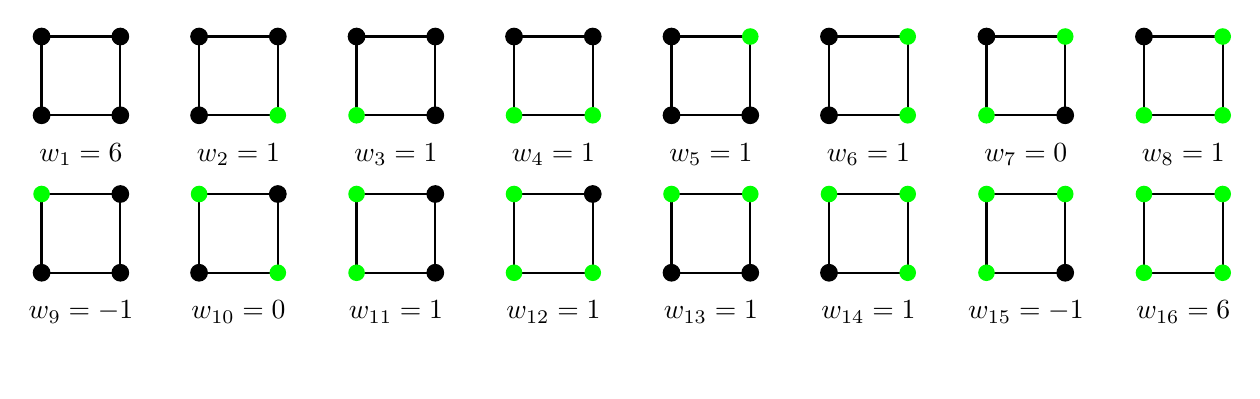
\begin{tikzpicture}
        % row1
        \cell{0}{0}{1}{1}
        \cell{2}{0}{3}{1}
        \cell{4}{0}{5}{1}
        \cell{6}{0}{7}{1}
        \cell{8}{0}{9}{1}
        \cell{10}{0}{11}{1}
        \cell{12}{0}{13}{1}
        \cell{14}{0}{15}{1}
        % row2
        \cell{0}{2}{1}{3}
        \cell{2}{2}{3}{3}
        \cell{4}{2}{5}{3}
        \cell{6}{2}{7}{3}
        \cell{8}{2}{9}{3}
        \cell{10}{2}{11}{3}
        \cell{12}{2}{13}{3}
        \cell{14}{2}{15}{3}
        % label for row1
        \draw[fill=black] (0,0) circle (3pt);
        \draw[fill=black] (1,0) circle (3pt);
        \draw[fill=black] (2,0) circle (3pt);
        \draw[fill=green, draw=none] (3,0) circle (3pt);
        \draw[fill=green, draw=none] (4,0) circle (3pt);
        \draw[fill=black] (5,0) circle (3pt);
        \draw[fill=green, draw=none] (6,0) circle (3pt);
        \draw[fill=green, draw=none] (7,0) circle (3pt);
        \draw[fill=black] (8,0) circle (3pt);
        \draw[fill=black] (9,0) circle (3pt);
        \draw[fill=black] (10,0) circle (3pt);
        \draw[fill=green, draw=none] (11,0) circle (3pt);
        \draw[fill=green, draw=none] (12,0) circle (3pt);
        \draw[fill=black] (13,0) circle (3pt);
        \draw[fill=green, draw=none] (14,0) circle (3pt);
        \draw[fill=green, draw=none] (15,0) circle (3pt);
        % label for row1
        \draw[fill=green, draw=none] (0,1) circle (3pt);
        \draw[fill=black] (1,1) circle (3pt);
        \draw[fill=green, draw=none] (2,1) circle (3pt);
        \draw[fill=black] (3,1) circle (3pt);
        \draw[fill=green, draw=none] (4,1) circle (3pt);
        \draw[fill=black] (5,1) circle (3pt);
        \draw[fill=green, draw=none] (6,1) circle (3pt);
        \draw[fill=black] (7,1) circle (3pt);
        \draw[fill=green, draw=none] (8,1) circle (3pt);
        \draw[fill=green, draw=none] (9,1) circle (3pt);
        \draw[fill=green, draw=none] (10,1) circle (3pt);
        \draw[fill=green, draw=none] (11,1) circle (3pt);
        \draw[fill=green, draw=none] (12,1) circle (3pt);
        \draw[fill=green, draw=none] (13,1) circle (3pt);
        \draw[fill=green, draw=none] (14,1) circle (3pt);
        \draw[fill=green, draw=none] (15,1) circle (3pt);
        % label for row1
        \draw[fill=black] (0,2) circle (3pt);
        \draw[fill=black] (1,2) circle (3pt);
        \draw[fill=black] (2,2) circle (3pt);
        \draw[fill=green, draw=none] (3,2) circle (3pt);
        \draw[fill=green, draw=none] (4,2) circle (3pt);
        \draw[fill=black] (5,2) circle (3pt);
        \draw[fill=green, draw=none] (6,2) circle (3pt);
        \draw[fill=green, draw=none] (7,2) circle (3pt);
        \draw[fill=black] (8,2) circle (3pt);
        \draw[fill=black] (9,2) circle (3pt);
        \draw[fill=black] (10,2) circle (3pt);
        \draw[fill=green, draw=none] (11,2) circle (3pt);
        \draw[fill=green, draw=none] (12,2) circle (3pt);
        \draw[fill=black] (13,2) circle (3pt);
        \draw[fill=green, draw=none] (14,2) circle (3pt);
        \draw[fill=green, draw=none] (15,2) circle (3pt);
        % label for row1
        \draw[fill=black] (0,3) circle (3pt);
        \draw[fill=black] (1,3) circle (3pt);
        \draw[fill=black] (2,3) circle (3pt);
        \draw[fill=black] (3,3) circle (3pt);
        \draw[fill=black] (4,3) circle (3pt);
        \draw[fill=black] (5,3) circle (3pt);
        \draw[fill=black] (6,3) circle (3pt);
        \draw[fill=black] (7,3) circle (3pt);
        \draw[fill=black] (8,3) circle (3pt);
        \draw[fill=green, draw=none] (9,3) circle (3pt);
        \draw[fill=black] (10,3) circle (3pt);
        \draw[fill=green, draw=none] (11,3) circle (3pt);
        \draw[fill=black] (12,3) circle (3pt);
        \draw[fill=green, draw=none] (13,3) circle (3pt);
        \draw[fill=black] (14,3) circle (3pt);
        \draw[fill=green, draw=none] (15,3) circle (3pt);
        % numbers row 1
        \( \lablnode{0.5}{-0.5}{$w_{9}=-1$} \)
        \( \lablnode{2.5}{-0.5}{$w_{10}=0$} \)
        \( \lablnode{4.5}{-0.5}{$w_{11}=1$} \)
        \( \lablnode{6.5}{-0.5}{$w_{12}=1$} \)
        \( \lablnode{8.5}{-0.5}{$w_{13}=1$} \)
        \( \lablnode{10.5}{-0.5}{$w_{14}=1$} \)
        \( \lablnode{12.5}{-0.5}{$w_{15}=-1$} \)
        \( \lablnode{14.5}{-0.5}{$w_{16}=6$} \)
        % numbers row 2
        \( \lablnode{0.5}{1.5}{$w_{1}=6$} \)
        \( \lablnode{2.5}{1.5}{$w_{2}=1$} \)
        \( \lablnode{4.5}{1.5}{$w_{3}=1$} \)
        \( \lablnode{6.5}{1.5}{$w_{4}=1$} \)
        \( \lablnode{8.5}{1.5}{$w_{5}=1$} \)
        \( \lablnode{10.5}{1.5}{$w_{6}=1$} \)
        \( \lablnode{12.5}{1.5}{$w_{7}=0$} \)
        \( \lablnode{14.5}{1.5}{$w_{8}=1$} \)
    \end{tikzpicture}
\end{center}

TODO

\end{proof}

\begin{theorem}
    \label{thm: growth rate}
    The growth rate of the main diagaonal $\gamma$ has 
    $$\gamma = \lim_{n \to \infty} \frac{t_{n+1,n+1}t_{n-1,n-1}}{t_{n,n}^2}$$
\end{theorem}


\section{Appendix}

Flipping the parity of a single vertex in a parity configuration changes the $4$ surrounding cells. This creates a constraint on a subset of $w_1 ,\dots, w_{16}.$ 

The flipping of parity of a single vertex can result in $2$ distinct types of constraints. Let a constraint of \textit{Type 1} be a parity flip that does not change the number of SAPs in the parity configuration. For example, consider the following flip of the center vertex in the following portion of a parity configuration.

\begin{center}
    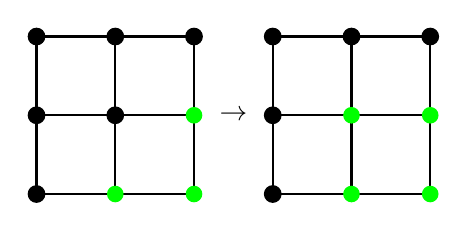
\begin{tikzpicture}
        % row1
        \cell{0}{0}{1}{1}
        \cell{1}{0}{2}{1}
        % row2
        \cell{0}{1}{1}{2}
        \cell{1}{1}{2}{2}
        % label for row1
        \draw[fill=black] (0,0) circle (3pt);
        \draw[fill=green, draw=none] (1,0) circle (3pt);
        \draw[fill=green, draw=none] (2,0) circle (3pt);
        % label for row2
        \draw[fill=black] (0,1) circle (3pt);
        \draw[fill=black] (1,1) circle (3pt);
        \draw[fill=green, draw=none] (2,1) circle (3pt);
        % label for row3
        \draw[fill=black] (0,2) circle (3pt);
        \draw[fill=black] (1,2) circle (3pt);
        \draw[fill=black] (2,2) circle (3pt);
        % row1
        \cell{3}{0}{4}{1}
        \cell{4}{0}{5}{1}
        % row2
        \cell{3}{1}{4}{2}
        \cell{4}{1}{5}{2}
        % label for row1
        \draw[fill=black] (3,0) circle (3pt);
        \draw[fill=green, draw=none] (4,0) circle (3pt);
        \draw[fill=green, draw=none] (5,0) circle (3pt);
        % label for row2
        \draw[fill=black] (3,1) circle (3pt);
        \draw[fill=green, draw=none] (4,1) circle (3pt);
        \draw[fill=green, draw=none] (5,1) circle (3pt);
        % label for row3
        \draw[fill=black] (3,2) circle (3pt);
        \draw[fill=black] (4,2) circle (3pt);
        \draw[fill=black] (5,2) circle (3pt);

        \( \lablnode{2.5}{1}{$\rightarrow$} \)
    \end{tikzpicture}
\end{center}

As this does not change the associated number of SAPs in the larger parity configuration, we want this to preserve the sign of the weight product. This gives the following associated constraint. 

$$\text{sign}(w_{1}w_{2}w_{5}w_{9}) = \text{sign}(w_{2}w_{4}w_{6}w_{16}).$$

Now let a constraint of \textit{Type 2} be a parity flip that does change the number of SAPs. For example, consider flipping the center vertex of the following portion of a parity configuration.

\begin{center}
    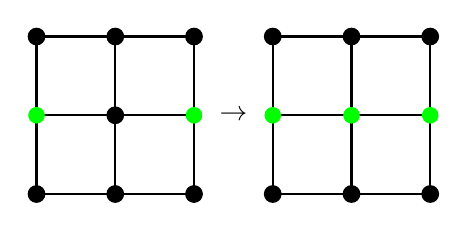
\begin{tikzpicture}
        % row1
        \cell{0}{0}{1}{1}
        \cell{1}{0}{2}{1}
        % row2
        \cell{0}{1}{1}{2}
        \cell{1}{1}{2}{2}
        % label for row1
        \draw[fill=black] (0,0) circle (3pt);
        \draw[fill=black] (1,0) circle (3pt);
        \draw[fill=black] (2,0) circle (3pt);
        % label for row2
        \draw[fill=green, draw=none] (0,1) circle (3pt);
        \draw[fill=black] (1,1) circle (3pt);
        \draw[fill=green, draw=none] (2,1) circle (3pt);
        % label for row3
        \draw[fill=black] (0,2) circle (3pt);
        \draw[fill=black] (1,2) circle (3pt);
        \draw[fill=black] (2,2) circle (3pt);
        % row1
        \cell{3}{0}{4}{1}
        \cell{4}{0}{5}{1}
        % row2
        \cell{3}{1}{4}{2}
        \cell{4}{1}{5}{2}
        % label for row1
        \draw[fill=black] (3,0) circle (3pt);
        \draw[fill=black] (4,0) circle (3pt);
        \draw[fill=black] (5,0) circle (3pt);
        % label for row2
        \draw[fill=green, draw=none] (3,1) circle (3pt);
        \draw[fill=green, draw=none] (4,1) circle (3pt);
        \draw[fill=green, draw=none] (5,1) circle (3pt);
        % label for row3
        \draw[fill=black] (3,2) circle (3pt);
        \draw[fill=black] (4,2) circle (3pt);
        \draw[fill=black] (5,2) circle (3pt);

        \( \lablnode{2.5}{1}{$\rightarrow$} \)
    \end{tikzpicture}
\end{center}

The above transformation corresponds with \textit{either} two distinct SAPs joining into one \textit{or} one SAP splitting into two distinct SAPs. In either case, we want the sign of the product to switch. This corresponds with the following constraint.

$$\text{sign}(w_{3}w_{2}w_{9}w_{5}) = -\text{sign}(w_{4}w_{4}w_{13}w_{13}).$$

All Type 1 constraints are as follows.

\begin{eqnarray*}
    w_{1}w_{1}w_{2}w_{3} = w_{2}w_{3}w_{6}w_{11} & w_{1}w_{1}w_{2}w_{4} = w_{2}w_{3}w_{6}w_{12} & w_{1}w_{1}w_{4}w_{3} = w_{2}w_{3}w_{8}w_{11} \\
    w_{1}w_{1}w_{4}w_{4} = w_{2}w_{3}w_{8}w_{12} & w_{1}w_{2}w_{1}w_{5} = w_{2}w_{4}w_{5}w_{13} & w_{1}w_{2}w_{1}w_{6} = w_{2}w_{4}w_{5}w_{14} \\
    w_{1}w_{2}w_{2}w_{8} = w_{2}w_{4}w_{6}w_{16} & w_{1}w_{2}w_{4}w_{8} = w_{2}w_{4}w_{8}w_{16} & w_{3}w_{1}w_{9}w_{1} = w_{4}w_{3}w_{13}w_{9} \\
    w_{3}w_{1}w_{11}w_{1} = w_{4}w_{3}w_{15}w_{9} & w_{3}w_{1}w_{12}w_{3} = w_{4}w_{3}w_{16}w_{11} & w_{3}w_{1}w_{12}w_{4} = w_{4}w_{3}w_{16}w_{12} \\
    w_{3}w_{2}w_{12}w_{8} = w_{4}w_{4}w_{16}w_{16} & w_{1}w_{6}w_{1}w_{5} = w_{2}w_{8}w_{5}w_{13} & w_{1}w_{6}w_{1}w_{6} = w_{2}w_{8}w_{5}w_{14} \\
    w_{1}w_{6}w_{2}w_{8} = w_{2}w_{8}w_{6}w_{16} & w_{1}w_{6}w_{4}w_{8} = w_{2}w_{8}w_{8}w_{16} & w_{3}w_{6}w_{12}w_{8} = w_{4}w_{8}w_{16}w_{16} \\
    w_{5}w_{9}w_{1}w_{1} = w_{6}w_{11}w_{5}w_{9} & w_{5}w_{13}w_{1}w_{1} = w_{6}w_{15}w_{5}w_{9} & w_{5}w_{14}w_{1}w_{5} = w_{6}w_{16}w_{5}w_{13} \\
    w_{5}w_{14}w_{1}w_{6} = w_{6}w_{16}w_{5}w_{14} & w_{5}w_{14}w_{2}w_{8} = w_{6}w_{16}w_{6}w_{16} & w_{5}w_{14}w_{4}w_{8} = w_{6}w_{16}w_{8}w_{16} \\
    w_{11}w_{1}w_{9}w_{1} = w_{12}w_{3}w_{13}w_{9} & w_{11}w_{1}w_{11}w_{1} = w_{12}w_{3}w_{15}w_{9} & w_{11}w_{1}w_{12}w_{3} = w_{12}w_{3}w_{16}w_{11} \\
    w_{11}w_{1}w_{12}w_{4} = w_{12}w_{3}w_{16}w_{12} & w_{11}w_{2}w_{12}w_{8} = w_{12}w_{4}w_{16}w_{16} & w_{11}w_{6}w_{12}w_{8} = w_{12}w_{8}w_{16}w_{16} \\
    w_{13}w_{9}w_{1}w_{1} = w_{14}w_{11}w_{5}w_{9} & w_{15}w_{9}w_{9}w_{1} = w_{16}w_{11}w_{13}w_{9} & w_{15}w_{9}w_{11}w_{1} = w_{16}w_{11}w_{15}w_{9} \\
    w_{15}w_{9}w_{12}w_{3} = w_{16}w_{11}w_{16}w_{11} & w_{15}w_{9}w_{12}w_{4} = w_{16}w_{11}w_{16}w_{12} & w_{13}w_{13}w_{1}w_{1} = w_{14}w_{15}w_{5}w_{9} \\
    w_{13}w_{14}w_{1}w_{5} = w_{14}w_{16}w_{5}w_{13} & w_{13}w_{14}w_{1}w_{6} = w_{14}w_{16}w_{5}w_{14} & w_{13}w_{14}w_{2}w_{8} = w_{14}w_{16}w_{6}w_{16} \\
    w_{13}w_{14}w_{4}w_{8} = w_{14}w_{16}w_{8}w_{16} & w_{15}w_{13}w_{9}w_{1} = w_{16}w_{15}w_{13}w_{9} & w_{15}w_{13}w_{11}w_{1} = w_{16}w_{15}w_{15}w_{9} \\
    w_{15}w_{13}w_{12}w_{3} = w_{16}w_{15}w_{16}w_{11} & w_{15}w_{13}w_{12}w_{4} = w_{16}w_{15}w_{16}w_{12} & w_{15}w_{14}w_{9}w_{5} = w_{16}w_{16}w_{13}w_{13} \\
    w_{15}w_{14}w_{9}w_{6} = w_{16}w_{16}w_{13}w_{14} & w_{15}w_{14}w_{11}w_{5} = w_{16}w_{16}w_{15}w_{13} & w_{15}w_{14}w_{11}w_{6} = w_{16}w_{16}w_{15}w_{14} \\
\end{eqnarray*}

Similarly, all Type 2 constraints are as follows.

\begin{eqnarray*}
        -w_{3}w_{2}w_{9}w_{5} = w_{4}w_{4}w_{13}w_{13} & -w_{3}w_{2}w_{9}w_{6} = w_{4}w_{4}w_{13}w_{14} & -w_{3}w_{2}w_{11}w_{5} = w_{4}w_{4}w_{15}w_{13} \\
        -w_{3}w_{2}w_{11}w_{6} = w_{4}w_{4}w_{15}w_{14} & -w_{3}w_{6}w_{9}w_{5} = w_{4}w_{8}w_{13}w_{13} & -w_{3}w_{6}w_{9}w_{6} = w_{4}w_{8}w_{13}w_{14} \\
        -w_{3}w_{6}w_{11}w_{5} = w_{4}w_{8}w_{15}w_{13} & -w_{3}w_{6}w_{11}w_{6} = w_{4}w_{8}w_{15}w_{14} & -w_{5}w_{9}w_{2}w_{3} = w_{6}w_{11}w_{6}w_{11} \\
        -w_{5}w_{9}w_{2}w_{4} = w_{6}w_{11}w_{6}w_{12} & -w_{5}w_{9}w_{4}w_{3} = w_{6}w_{11}w_{8}w_{11} & -w_{5}w_{9}w_{4}w_{4} = w_{6}w_{11}w_{8}w_{12} \\
        -w_{5}w_{13}w_{2}w_{3} = w_{6}w_{15}w_{6}w_{11} & -w_{5}w_{13}w_{2}w_{4} = w_{6}w_{15}w_{6}w_{12} & -w_{5}w_{13}w_{4}w_{3} = w_{6}w_{15}w_{8}w_{11} \\
        -w_{5}w_{13}w_{4}w_{4} = w_{6}w_{15}w_{8}w_{12} & -w_{11}w_{2}w_{9}w_{5} = w_{12}w_{4}w_{13}w_{13} & -w_{11}w_{2}w_{9}w_{6} = w_{12}w_{4}w_{13}w_{14} \\
        -w_{11}w_{2}w_{11}w_{5} = w_{12}w_{4}w_{15}w_{13} & -w_{11}w_{2}w_{11}w_{6} = w_{12}w_{4}w_{15}w_{14} & -w_{11}w_{6}w_{9}w_{5} = w_{12}w_{8}w_{13}w_{13} \\
        -w_{11}w_{6}w_{9}w_{6} = w_{12}w_{8}w_{13}w_{14} & -w_{11}w_{6}w_{11}w_{5} = w_{12}w_{8}w_{15}w_{13} & -w_{11}w_{6}w_{11}w_{6} = w_{12}w_{8}w_{15}w_{14} \\
        -w_{13}w_{9}w_{2}w_{3} = w_{14}w_{11}w_{6}w_{11} & -w_{13}w_{9}w_{2}w_{4} = w_{14}w_{11}w_{6}w_{12} & -w_{13}w_{9}w_{4}w_{3} = w_{14}w_{11}w_{8}w_{11} \\
        -w_{13}w_{9}w_{4}w_{4} = w_{14}w_{11}w_{8}w_{12} & -w_{13}w_{13}w_{2}w_{3} = w_{14}w_{15}w_{6}w_{11} & -w_{13}w_{13}w_{2}w_{4} = w_{14}w_{15}w_{6}w_{12} \\
        -w_{13}w_{13}w_{4}w_{3} = w_{14}w_{15}w_{8}w_{11} & -w_{13}w_{13}w_{4}w_{4} = w_{14}w_{15}w_{8}w_{12} & 
\end{eqnarray*}

Solving all Type 1 and Type 2 constrains gives the following solution set.

\begin{eqnarray*}
    [w_{1}, ..., w_{16}] & = & [6, -1, -1, -1, -1, -1, 0, -1, 1, 0, -1, -1, -1, -1, 1, 6] \\
    & = & [6, -1, -1, -1, -1, 1, 0, 1, 1, 0, 1, 1, -1, 1, -1, 6] \\
    & = & [6, -1, -1, -1, 1, -1, 0, -1, -1, 0, -1, -1, -1, 1, -1, 6] \\
    & = & [6, -1, -1, -1, 1, 1, 0, 1, -1, 0, 1, 1, -1, -1, 1, 6] \\
    & = & [6, -1, -1, 1, -1, -1, 0, 1, 1, 0, -1, 1, 1, 1, -1, 6] \\
    & = & [6, -1, -1, 1, -1, 1, 0, -1, 1, 0, 1, -1, 1, -1, 1, 6] \\
    & = & [6, -1, -1, 1, 1, -1, 0, 1, -1, 0, -1, 1, 1, -1, 1, 6] \\
    & = & [6, -1, -1, 1, 1, 1, 0, -1, -1, 0, 1, -1, 1, 1, -1, 6] \\
    & = & [6, -1, 1, -1, -1, -1, 0, -1, -1, 0, -1, 1, -1, -1, -1, 6] \\
    & = & [6, -1, 1, -1, -1, 1, 0, 1, -1, 0, 1, -1, -1, 1, 1, 6] \\
    & = & [6, -1, 1, -1, 1, -1, 0, -1, 1, 0, -1, 1, -1, 1, 1, 6] \\
    & = & [6, -1, 1, -1, 1, 1, 0, 1, 1, 0, 1, -1, -1, -1, -1, 6] \\
    & = & [6, -1, 1, 1, -1, -1, 0, 1, -1, 0, -1, -1, 1, 1, 1, 6] \\
    & = & [6, -1, 1, 1, -1, 1, 0, -1, -1, 0, 1, 1, 1, -1, -1, 6] \\
    & = & [6, -1, 1, 1, 1, -1, 0, 1, 1, 0, -1, -1, 1, -1, -1, 6] \\
    & = & [6, -1, 1, 1, 1, 1, 0, -1, 1, 0, 1, 1, 1, 1, 1, 6] \\
    & = & [6, 1, -1, -1, -1, -1, 0, 1, -1, 0, -1, -1, -1, -1, -1, 6] \\
    & = & [6, 1, -1, -1, -1, 1, 0, -1, -1, 0, 1, 1, -1, 1, 1, 6] \\
    & = & [6, 1, -1, -1, 1, -1, 0, 1, 1, 0, -1, -1, -1, 1, 1, 6] \\
    & = & [6, 1, -1, -1, 1, 1, 0, -1, 1, 0, 1, 1, -1, -1, -1, 6] \\
    & = & [6, 1, -1, 1, -1, -1, 0, -1, -1, 0, -1, 1, 1, 1, 1, 6] \\
    & = & [6, 1, -1, 1, -1, 1, 0, 1, -1, 0, 1, -1, 1, -1, -1, 6] \\
    & = & [6, 1, -1, 1, 1, -1, 0, -1, 1, 0, -1, 1, 1, -1, -1, 6] \\
    & = & [6, 1, -1, 1, 1, 1, 0, 1, 1, 0, 1, -1, 1, 1, 1, 6] \\
    & = & [6, 1, 1, -1, -1, -1, 0, 1, 1, 0, -1, 1, -1, -1, 1, 6] \\
    & = & [6, 1, 1, -1, -1, 1, 0, -1, 1, 0, 1, -1, -1, 1, -1, 6] \\
    & = & [6, 1, 1, -1, 1, -1, 0, 1, -1, 0, -1, 1, -1, 1, -1, 6] \\
    & = & [6, 1, 1, -1, 1, 1, 0, -1, -1, 0, 1, -1, -1, -1, 1, 6] \\
    & = & [6, 1, 1, 1, -1, -1, 0, -1, 1, 0, -1, -1, 1, 1, -1, 6] \\
    & = & [6, 1, 1, 1, -1, 1, 0, 1, 1, 0, 1, 1, 1, -1, 1, 6] \\
    & = & [6, 1, 1, 1, 1, -1, 0, -1, -1, 0, -1, -1, 1, -1, 1, 6] \\
    & = & [6, 1, 1, 1, 1, 1, 0, 1, -1, 0, 1, 1, 1, 1, -1, 6] \\
\end{eqnarray*}

Any of these assignments are sufficient for calculating $t_{n,m}$. 

\section{Bibliography}

TODO

\end{document}